\begin{theorem}
    Пусть $K$~---~компакт, $K \neq \varnothing$. Пусть $f$: $K \mapsto R$. Если $f$~---~полунепрерывна снизу на компакте, то она достигает своего минимума, а если полунепрерывна сверху, то~---~максимума.
\end{theorem}
\begin{proof}
    Докажем для полунепрерывности сверху, так как для полунепрерывности снизу доказательство аналогично. 
    
    Пусть $f (K) := \{ f (x)$: $x \in K\} \subset \R$. Тогда $\exists \sup f (K) = M.$ Пока знаем, что $M \in \overline{\R}$. Из \hyperlink{prop4.2}{утверждения 4.2} получаем: $\forall n \in \N \  \exists y_{n} \in f (K)$: $y_{n} \in U_{\frac{1}{n}} (M)$. Но тогда $\forall n \in \N \ \exists x_{n} \in K$: $f (x_{n}) \in U_{\frac{1}{n}} (M) \Rightarrow$ построили последовательность точек $\{ x_{n} \} \subset K$: $f (x_{n}) \to M, \ n \to \infty$. (Примечание: обычно такая последовательность называется <<максимизирующая>>)

    Так как $K$~---~компакт, то существует подпоследовательность $\{ x_{n_{j}} \}$ последовательности $\{ x_{n} \}$ и точка $x^{*} \in K$: $x_{n_{j}} \to x^{*}, j \to \infty$. Но $f$~---~полунепрерывна сверху в точке $x^{*} \Rightarrow \overline{\lim\limits_{j\to \infty}} f (x_{n_{j}}) \leq \overline{\lim\limits_{\underset{x \in K}{x\to x^{*}}}} f (x) \leq f (x^{*})$. Но на самом деле $\overline{\lim\limits_{j\to \infty}} f (x_{n_{j}}) = \lim\limits_{j\to \infty} f (x_{n_{j}}) = M.$ А тогда $f (x^{*}) \geq M$, но $f (x^{*}) \in f (K) \Rightarrow f (x^{*}) \leq M.$ Итого получаем, $f (x^{*}) = M$. То есть она достигает максимума.
\end{proof} %что тебе опять не так?
\begin{corollary}
    Если функция непрерывна на непустом компакте $K$, то она достигает и максимума, и минимума. В частности, функция непрерывная на отрезке достигает на нём своего максимума и минимума.
\end{corollary}

\textbf{Введём следующие обозначения:} если $f$: $E \mapsto \R$ и непрерывна на нём, то $f \in \text{C} (E).$

\begin{theorem}
    \hypertarget{thm5.4}{(Теорема Больцано-Коши/о промежуточном значении) Пусть} $a < b$. Пусть $f \in \text{C} ([a, b])$. Тогда $\forall y^{*} \in [min\big[f (a), f (b)\big], max\big[f (a), f (b)\big]]\  \exists x^{*} \in [a, b]$: $f (x^{*}) = y^{*}.$
\end{theorem}

\begin{proof}

    Для удобства доказательства положим $f (a) < f (b)$, в противном случае доказательство не изменится с точностью до знаков.

    \underline{Примечание.} В доказательстве запись $[l, r]$ подразумевает отрезок $[min(l, r), max(l, r)]$. Опять же исключительно для удобства записи мы так сокращаем.

    Пусть $[a, b] = I^{0}$. Поделим $I^{0}$ пополам, то есть рассмотрим $c_{1} = \frac{a + b}{2}$. 
    
    Возможно 2 варианта: $
    \left[
    \begin{gathered}
        y^{*} \in [f (c_{1}), f (b)];\\
        y^{*} \in [f (a), f (c_{1})].
    \end{gathered}
    \right.
    $
    Выберем такую половину $I^{0}$, что $y^{*}$ принадлежит отрезку, образованному значениями $f$ в концах половинок, назовём его $I^{1}$. Такой отрезок обязательно найдётся, иначе мы бы пришли к противоречию с тем, что $y^{*} \in I^{0}$.

    Пусть построено $k + 1$ отрезков: $I^{0} \supset I^{1} \supset \ldots \supset I^{k}$. $I^{k} = [a_{k}, b_{k}]$, при этом $y^{*} \in [a_{j}, b_{j}] \  \forall j \in \{0, 1, \ldots, k\}$.
    $|I^{j}| = \frac{|b - a|}{2^{j}} \  \forall j \in \{ 0, 1, \ldots, k\}$. 
    
    
\sidefig(10 cm)(7 cm)
{
\begin{flushleft}
    На $k + 1$ шаге делим $I^{k}$ пополам. Пусть $c_{k + 1} = \frac{a_{k} + b_{k}}{2}$. Возможно 2 случая: $
    \left[
    \begin{gathered}
        y^{*} \in [f (c_{k + 1}), f (b_{k})];\\
        y^{*} \in [f (a_{k}), f (c_{k + 1})].
    \end{gathered}
    \right.
    $

     Обязательно найдётся половина, для которой $y^{*}$ будет принадлежать отрезку, образованному значениями функции в концах этой половины, иначе $y^{*} \notin [a_{k}, b_{k}]$, что противоречит построению.
\end{flushleft}
}
{
    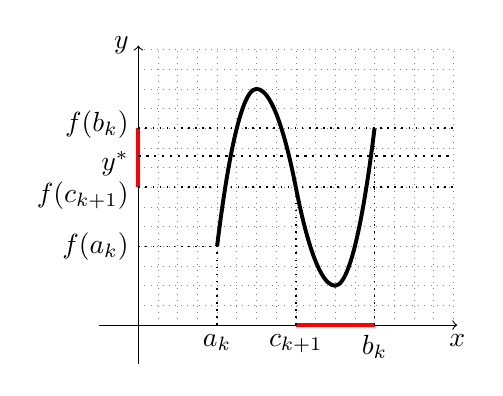
\begin{tikzpicture}
    % Рисуем сетку
    \draw[help lines, step=0.25, dotted]
    (-2,-2) grid (2,1.5);
    % Начало координат
    \draw[->, thin] (-2.5,-2) -- (2.05,-2)
    node[below] {$x$}; % Ox
    \draw[->, thin] (-2,-2.5) -- (-2,1.55)
    node[left] {$y$}; % Oy

    \draw[line width =.05cm](-1, -1) parabola bend (-0.5, 1) (0, -0.25);
    \draw[line width =.05cm](0, -0.25) parabola bend (0.5, -1.5) (1, 0.5);

    \draw[line width =.05cm, red] (1, -2) -- (0,-2);
    \draw[line width =.05cm, red] (-2, -0.25) -- (-2, 0.5);

    \draw[dotted, line width =.02cm] (-1, -2) -- (-1, -1);
    \draw[dotted, line width =.02cm] (0, -2) -- (0, -0.25);
    \draw[dotted, line width =.02cm] (1, -2) -- (1, 0.5);
    \draw[dotted, line width =.02cm] (-2, -1) -- (-1, -1);
    \draw[dotted, line width =.02cm] (-2, -0.25) -- (2, -0.25);
    \draw[dotted, line width =.02cm] (-2, 0.5) -- (2, 0.5);
    \draw[dotted, line width =.03cm] (-2, 0.15) -- (2, 0.15);

    \node[left] at (-2, 0.05) {$y^{*}$};
    \node[left] at (-2, 0.55) {$f(b_{k})$};
    \node[left] at (-2, -1) {$f(a_{k})$};
    \node[left] at (-2, -0.35) {$f(c_{k+1})$};
    \node[below] at (-1, -2) {$a_{k}$};
    \node[below] at (0, -2) {$c_{k+1}$};
    \node[below] at (1, -2) {$b_{k}$};
    \end{tikzpicture}
}

По индукции мы построили стягивающуюся последовательность вложенных отрезков $\displaystyle \{ I^{k} \}^{\infty}_{k = 1} \Rightarrow \exists ! x^{*} = \bigcap^{\infty}_{k = 1} I^{k}$. По построению $\forall k \in \N \  y^{*} \in [f (a_{k}), f (b_{k})]$.
    
Но $f$ непрерывна в точке $x^{*}$, то есть $a_{k}\to x^{*}, \ k \to \infty$ и $b_{k}\to x^{*}, \  k \to \infty \Rightarrow f (a_{k})\to f(x^{*}), \ k \to \infty$ и $f (b_{k})\to f(x^{*}), \  k \to \infty.$ Тогда по теореме о двух миллиционерах и так как $y^{*}$~---~стационарная последовательность, то $y^{*} = f (x^{*})$.

\end{proof}
\begin{definition}
    \textit{Промежутком} назовём либо отрезок, либо инвервал, либо полуинтервал, то есть $\lfloor a, b\rceil \Leftrightarrow$ $[a, b]$ или $(a, b)$, или $[a, b)$, или $(a, b]$.
\end{definition}
\begin{theorem}
    \hypertarget{thrm4.15}{(Обобщённая теорема о промежуточном значении)} Пусть $f$: $\lfloor a, b\rceil \mapsto \R$. Пусть $f \in \text{C} \big(\lfloor a, b\rceil \big)$. Пусть $m = \underset{x \in \lfloor a, b\rceil}{\inf} f (x)$, $M = \underset{x \in \lfloor a, b\rceil}{\sup} f (x)$. Тогда $\forall y^{*} \in (m, M) \  \exists x^{*} \in \lfloor a, b\rceil$: $f (x^{*}) = y^{*}$.
\end{theorem} 
\begin{proof}
    По определению инфимума $\exists a_{1} \in \lfloor a, b\rceil$: $m \leq f (a_{1}) < y^{*}$. Аналогично по определению супремума $\exists b_{1} \in \lfloor a, b\rceil$: $M \geq f (b_{1}) > y^{*}.$ Следовательно $y^{*} \in [f (a_{1}), f (b_{1})]$. И при этом $f \in \text{C} \big( [a_{1}, b_{1} ]\big) \Rightarrow$ по \hyperlink{thm5.4}{теореме Больцано-Коши} $\exists x^{*} \in [a_{1}, b_{1}]$: $f (x^{*}) = y^{*}$, что и требовалось.
\end{proof}
\begin{corollary}
    Если $f \in \text{C} \big([a, b]\big)$, то $f \big( [a, b] \big) = [\underset{x \in [a, b]}{min} f (x), \underset{x \in [a, b]}{max} f (x)].$
\end{corollary}
\begin{proof}
    Было доказано, что (так как $f$ непрерывна на $[a, b]$, а отрезок компакт) $\exists x_{m} \in [a, b]$: $\forall x \in [a, b] \hookrightarrow f (x) \geq f (x_{m})$ и $\exists x_{M} \in [a, b]$: $\forall x \in [a, b] \hookrightarrow f (x_{M}) \geq f (x)$.

    Получается, $\forall x \in [a, b] \hookrightarrow f (x) \in [f (x_{m}), f (x_{M})]$. Но по \hyperlink{thm5.4}{теореме Больцано-Коши} получаем сюръекцию (все значения принимаются), то есть $\forall y \in [f (x_{m}, f (x_{M})] \  \exists x \in [a, b]$: $f (x) = y$. Значит $f \big( [a, b] \big) = [f (x_{m}), f (x_{M})]$.
\end{proof}
\begin{problem}
    Верно ли, что образ интервала~---~интервал?
\end{problem}
\begin{solution}
    Нет. К примеру, $f (x) = \sin (x)$, $x \in (-\pi, \pi)$. Но для монотонных функций это верно.
\end{solution}
\subsection{Колебания}
\begin{definition}
    Пусть $E \subset \R$, $E \neq \varnothing$. Пусть $f$: $E \mapsto \R$.
    
    \textit{Колебание $f$ на $E$}~---~$\omega_{E} [f] := \underset{x_{1}, x_{2} \in E}{\sup} |f (x_{1}) - f (x_{2})|$.
\end{definition}
\begin{definition}
    Пусть $X \subset \R$, $X \neq \varnothing$, $x_{0} \in X$. Тогда \textit{колебанием функции в точке} назовём $\omega_{x_{0}} [f] := \underset{\delta > 0}{\inf} \omega_{U_{\delta} (x_{0})} [f]$.
\end{definition}
\begin{theorem}
    \hypertarget{thm4.16}{Функция непрерывна в точке по множеству} $\Leftrightarrow$ колебание в ней 0. То есть пусть $X \subset \R$, $X \neq \varnothing$, $x_{0} \in X$, $f$~---~непрерывна в точке $x_{0}$ по множеству $X \Leftrightarrow \omega_{x_{0}} [f] = 0.$
\end{theorem}
\begin{proof}
    \underline{Шаг 1.} Пусть $f$ непрерывна в точке $x_{0} \Rightarrow \forall \epsilon > 0 \  \exists \delta (\epsilon) > 0$: $\forall x \in U_{\delta} (x_{0}) \cap X \hookrightarrow |f (x) - f (x_{0})| < \frac{\epsilon}{2}$. Тогда $\forall \epsilon > 0 \  \exists \delta (\epsilon) > 0$: $\forall x_{1}, x_{2} \in U_{\delta} (x_{0} \cap X \hookrightarrow |f (x_{1}) - f (x_{2})| < \epsilon$ по неравенству треугольника.

    Получается $\forall \epsilon > 0 \  \exists \delta (\epsilon)$: $\omega_{U_{\delta (\epsilon)} (x_{0}) \cap X} [f] \leq \epsilon$, но так как есть монотонность по $\delta$, то $\exists \lim\limits_{\delta\to +0} \omega_{U_{\delta (\epsilon)} (x_{0}) \cap X} [f] = 0 = \underset{\delta > 0}{\inf} \omega_{U_{\delta (\epsilon)} (x_{0}) \cap X} [f]$ по \hyperlink{thm4.5}{теореме Вейерштрасса}. В одну сторону доказали.

    \underline{Шаг 2.} Пусть $\omega_{x_{0}} [f] = 0$. Покажем непрерывность.

    В силу монотонности $\omega_{U_{\delta (\epsilon)} (x_{0}) \cap X} [f]$ по $\delta$ получаем, что $\exists \lim\limits_{\delta\to +0} \omega_{U_{\delta (\epsilon)} (x_{0}) \cap X} [f] = 0$. Тогда по определению получаем:
    $$ \forall \epsilon > 0 \  \exists \delta (\epsilon) > 0: \forall \delta \in \big(0, \delta (\epsilon)\big] \hookrightarrow \omega_{U_{\delta (\epsilon)} (x_{0}) \cap X} [f] < \epsilon.$$

    Тогда, взяв $x_{1} = x_{0}$, а $\delta = \delta (\epsilon)$, получим
    $$\forall \epsilon > 0 \  \exists \delta (\epsilon) > 0: \underset{x_{2} \in U_{\delta (\epsilon)} (x_{0}) \cap X}{\sup} |f (x_{2}) - f (x_{0})| < \epsilon \Rightarrow f\text{~---~непрерывна в точке } x_{0}.$$
\end{proof}
\begin{note}
    Можно легко доказать разрывность функции Дирихле в каждой точке.

    Заметим, что $\forall \underline{x} \in \R$ $\omega_{U_{\delta} (\underline{x})} [D] = 1$, поскольку любой невырожденный интервал на числовой прямой содержит как рациональные, так иррациональные точки $\Rightarrow \omega_{\underline{x}} [D] = 1$ $\forall \underline{x} \in \R$, а значит по \hyperlink{thm4.16}{теореме 4.16} функция Дирихле разрывна в каждой точке.
\end{note}
\begin{definition}
    \textit{Функцией Римана} назовём:
    $$
    R (x) := \begin{cases}
        0, \  \forall x \in \R \backslash \Q \\
        \frac{1}{q}, \  \forall x \in \Q \ (x = \frac{p}{q}, \ p \in \Z, \ q \in \N, \ (p, q) = 1)
    \end{cases}
    $$
\end{definition}
\begin{problem}
    Доказать, что функция Римана непрерывна в $\R \backslash \Q$ и разрывна в $\Q$.
\end{problem}
\begin{solution}
    Поскольку в любой окрестности любой точки содержатся иррациональные числа, получаем
    $$ \omega_{x} [R] \geq \frac{1}{q} \quad  \forall x \in \Q.$$

    Тогда в силу \hyperlink{thm4.16}{теоремы 4.16} получаем, что функция Римана разрывна в каждой рациональной точке.

    Покажем, что функция Римана непрерывна в каждой иррациональной точке. Зафиксируем $\underline{x} \in \R \backslash \Q$. Заметим, что $\forall q \in \N \ \exists \delta (\underline{x}, q) > 0$: $U_{\delta (\underline{x}, q)} (\underline{x})$ не содержит несократимых дробей со знаменателями $q' \in \{ 1, \ldots, q \}$. Действительно, положим
    $$ \delta (\underline{x}, q) := min \{ |\underline{x} - \frac{p'}{q'}|: 1 \leq q' \leq q, \frac{p'}{q'}\text{~---~несократимая дробь.}\}$$

    Но тогда получается, что $R (\underline{x}) - R (x) = 0 \  \forall x \in (\R \backslash \Q) \cap U_{\delta (\underline{x}, q)} (\underline{x})$. Если же $x \in \Q \cap U_{\delta (\underline{x}, q)} (\underline{x})$, то $| R (\underline{x}) - R (x)| < \frac{1}{q}$. В итоге получаем, что $\forall n \in \N \forall \underline{x} \in \R \backslash \Q \  \exists \delta (\underline{x}, n) > 0$: $\omega_{U_{\delta (\underline{x}, n)} (\underline{x})} [R] < \frac{1}{n}$. Отсюда получаем
    $$ \omega_{x} [R] = 0 \  \forall x \in \R \backslash \Q.$$
\end{solution}
\begin{problem}
    Доказать, что не существует функции, непрерывной в $\Q$ и разрывной в $\R \backslash \Q$.
\end{problem}
\begin{theorem} \hypertarget{thrm4.17}{(О замене переменной под знаком предела)}
    Пусть $x_{0}, y_{0} \in \overline{\R}$. Пусть $y$: $\mathring{U}_{\delta_{0}} (x_{0}) \mapsto \R$, $f$: $\mathring{U}_{\delta_{0}} (y_{0}) \mapsto \R$. 
    
    Пусть $\exists \lim\limits_{y\to y_{0}} f (y) = A$, $A \in \Hat{\R}$ и $y (x) \neq y_{0} \  \forall x \in \mathring{U}_{\delta_{0}} (x_{0}).$ Тогда $\exists \lim\limits_{x\to x_{0}} f (y (x)) = A.$
\end{theorem}
\begin{proof}
    Зафиксируем произвольное $\epsilon > 0$. Так как $\lim_{y \to y_{0}} f (y) = A$, то
    $$ \exists \beta \in (0; \beta_{0}): \forall y \in \ring{U}_{\beta} (y_{0}) \hookrightarrow f (y) \in U_{\epsilon} (A).$$
    По определению предела
\end{proof}